\documentclass[11pt]{article}

\usepackage{amsmath}
\usepackage{booktabs}
\usepackage{braket}
\usepackage{chemfig}
\usepackage{chemformula}
\usepackage[outline]{contour}
\usepackage{enumitem}
\usepackage[T1]{fontenc}
\usepackage[margin=1in]{geometry}
\usepackage{graphicx}
\usepackage[utf8]{inputenc}
\usepackage{libertine}
\usepackage{mathtools}
\usepackage[libertine]{newtxmath}
\usepackage{pgfplots}
\usepackage[detect-weight=true]{siunitx}

\title{PHYS 234 Assignment 2}
\author{Brandon Tsang}
\date{May 29, 2020}

\pgfplotsset{compat=1.17}
\contourlength{0.1em}
\newcommand\uline[1]{\underline{\smash{#1}}\llap{\contour{white}{#1}}}
\DeclarePairedDelimiter\abs{\lvert}{\rvert}
\makeatletter
\let\oldabs\abs
\def\abs{\@ifstar{\oldabs}{\oldabs*}}
\let\oldnorm\norm
\def\norm{\@ifstar{\oldnorm}{\oldnorm*}}
\makeatother

\newenvironment{amatrix}[1]{%
    \left[\begin{array}{@{}*{#1}{c}|c@{}}
}{%
    \end{array}\right]
}

\begin{document}
    \maketitle
    \begin{enumerate}[label=\textbf{\arabic*.}]
        \item{
            \textbf{\boldmath \uline{Computing Probabilities} \\ A beam of spin-\(\tfrac 1 2\) particles is prepared in the state \[\ket{\psi}=\tfrac{3i}{5}\ket{+}_y+\tfrac 4 5\ket{-}_y.\]}%
            The state is given in terms of the \(S_y\) eigenvectors. Since we derived relations for the \(S_z\) operator in class, I will express \(\ket \psi\) in terms of \(S_z\) eigenvectors to ease the calculations.
            \par
            First, I will confirm that \(\ket \psi\) is normalized:
            \begin{align*}
                \braket{\psi|\psi}&\stackrel{?}{=}1 \\
                \left(-\tfrac{3i}{5}\prescript{}{y}{\bra{+}}+\tfrac 4 5\prescript{}{y}{\bra{-}}\right)\left(\tfrac{3i}{5}\ket{+}_y+\tfrac 4 5\ket{-}_y\right)&\stackrel{?}{=}1 \\
                \frac{9}{25}+\frac{16}{25}&\stackrel{?}{=}1 \\
                1&=1
            \end{align*}
            Then, I find the projection of \(\ket \psi\) onto \(\ket +\):
            \begin{align*}
                \braket{+|\psi}&=\bra{+}\left(\tfrac{3i}{5}\ket{+}_y+\tfrac 4 5\ket{-}_y\right) \\
                &=\tfrac{3i}{5}\braket{+|+}_y+\tfrac 4 5 \braket{+|-}_y
            \end{align*}
            From class, \(\ket{+}_y=\frac{1}{\sqrt 2}(\ket{+}+i\ket{-})\) and \(\ket{-}_y=\frac{1}{\sqrt 2}(\ket{+}-i\ket{-})\):
            \begin{align*}
                &=\tfrac{3i}{5}\bra{+}\cdot\tfrac{1}{\sqrt 2}(\ket{+}+i\ket{-})+\tfrac 4 5 \bra{+}\cdot\tfrac{1}{\sqrt 2}(\ket{+}-i\ket{-}) \\
                &=\tfrac{3i}{5\sqrt 2}(\braket{+|+}+i\braket{+|-})+\tfrac{4}{5\sqrt 2}(\braket{+|+}-i\braket{+|-}) \\
                &=\frac{4+3i}{5\sqrt 2}
            \end{align*}
            And again with \(\ket -\):
            \begin{align*}
                \braket{-|\psi}&=\bra{-}\left(\tfrac{3i}{5}\ket{+}_y+\tfrac 4 5\ket{-}_y\right) \\
                &=\tfrac{3i}{5}\braket{-|+}_y+\tfrac 4 5 \braket{-|-}_y \\
                &=\tfrac{3i}{5}\bra{-}\cdot\tfrac{1}{\sqrt 2}(\ket{+}+i\ket{-})+\tfrac 4 5 \bra{-}\cdot\tfrac{1}{\sqrt 2}(\ket{+}-i\ket{-}) \\
                &=\tfrac{3i}{5\sqrt 2}(\braket{-|+}+i\braket{-|-})+\tfrac{4}{5\sqrt 2}(\braket{-|+}-i\braket{-|-}) \\
                &=\frac{3i^2}{5\sqrt 2}-\frac{4i}{5\sqrt 2} \\
                &=\frac{-3-4i}{5\sqrt 2}
            \end{align*}
            So \(\ket \psi\) is then \[\ket \psi=\tfrac{1}{5\sqrt 2}((4+3i)\ket{+}-(3+4i)\ket{-}).\]
            \begin{enumerate}[label=\textbf{(\alph*)}]
                \item{
                    \textbf{\boldmath What are the possible measurement results of the spin operator \(S_x\) and with what probability would they occur?}
                    \par
                    The two possible measurement results are \(+\frac \hbar 2\) and \(-\frac \hbar 2\).
                    \par
                    The probability of \(+\frac \hbar 2\) is:
                    \begin{align*}
                        \abs{\prescript{}{x}{\braket{+|\psi}}}^2&=\abs{\prescript{}{x}{\bra{+}}\cdot\tfrac{1}{5\sqrt 2}((4+3i)\ket{+}-(3+4i)\ket{-})}^2 \\
                        &=\abs{\tfrac{4+3i}{5\sqrt 2}\prescript{}{x}{\braket{+|+}}-\tfrac{3+4i}{5\sqrt 2}\prescript{}{x}{\braket{+|-}}}^2
                    \end{align*}
                    From class, \(\ket{+}_x=\frac{1}{\sqrt 2}(\ket{+}+\ket{-})\):
                    \begin{align*}
                        &=\abs{\tfrac{4+3i}{5\sqrt 2}\cdot\tfrac{1}{\sqrt 2}(\bra{+}+\bra{-})\ket{+}-\tfrac{3+4i}{5\sqrt 2}\cdot\tfrac{1}{\sqrt 2}(\bra{+}+\bra{-})\ket{-}}^2 \\
                        &=\abs{\frac{4+3i}{5\cdot 2}-\frac{3+4i}{5\cdot 2}}^2 \\
                        &=\abs{\frac{1-i}{10}}^2 \\
                        &=\frac{1+1}{100} \\
                        &=\frac{1}{50}
                    \end{align*}
                    The probability of \(-\frac \hbar 2\) is:
                    \begin{align*}
                        \abs{\prescript{}{x}{\braket{-|\psi}}}^2&=\abs{\prescript{}{x}{\bra{+}}\cdot\tfrac{1}{5\sqrt 2}((4+3i)\ket{+}-(3+4i)\ket{-})}^2 \\
                        &=\abs{\tfrac{4+3i}{5\sqrt 2}\prescript{}{x}{\braket{-|+}}-\tfrac{3+4i}{5\sqrt 2}\prescript{}{x}{\braket{-|-}}}^2
                    \end{align*}
                    From class, \(\ket{-}_x=\frac{1}{\sqrt 2}(\ket{+}-\ket{-})\):
                    \begin{align*}
                        &=\abs{\tfrac{4+3i}{5\sqrt 2}\cdot\tfrac{1}{\sqrt 2}(\bra{+}-\bra{-})\ket{+}-\tfrac{3+4i}{5\sqrt 2}\cdot\tfrac{1}{\sqrt 2}(\bra{+}-\bra{-})\ket{-}}^2 \\
                        &=\abs{\frac{4+3i}{5\cdot 2}+\frac{3+4i}{5\cdot 2}}^2 \\
                        &=\abs{\frac{7-7i}{10}}^2 \\
                        &=\frac{49+49}{100} \\
                        &=\frac{49}{50}
                    \end{align*}
                }
                \item{
                    \textbf{\boldmath What are the possible measurement results of the spin operator \(S_y\) and with what probability would they occur?}
                    \par
                    The two possible measurement results are \(+\frac \hbar 2\) and \(-\frac \hbar 2\).
                    \par
                    The probability of \(+\frac \hbar 2\) is:
                    \begin{align*}
                        \abs{\prescript{}{y}{\braket{+|\psi}}}^2&=\abs{\prescript{}{y}{\bra{+}}\cdot\tfrac{1}{5\sqrt 2}((4+3i)\ket{+}-(3+4i)\ket{-})}^2 \\
                        &=\abs{\tfrac{4+3i}{5\sqrt 2}\prescript{}{y}{\braket{+|+}}-\tfrac{3+4i}{5\sqrt 2}\prescript{}{y}{\braket{+|-}}}^2
                    \end{align*}
                    From class, \(\ket{+}_y=\frac{1}{\sqrt 2}(\ket{+}+i\ket{-})\):
                    \begin{align*}
                        &=\abs{\tfrac{4+3i}{5\sqrt 2}\cdot\tfrac{1}{\sqrt 2}(\bra{+}+i\bra{-})\ket{+}-\tfrac{3+4i}{5\sqrt 2}\cdot\tfrac{1}{\sqrt 2}(\bra{+}+i\bra{-})\ket{-}}^2 \\
                        &=\abs{\frac{4+3i}{5\cdot 2}-\frac{3+4i}{5\cdot 2}i}^2 \\
                        &=\abs{\frac{4+3i}{5\cdot 2}-\frac{-4+3i}{5\cdot 2}}^2 \\
                        &=\abs{\frac{8}{10}}^2 \\
                        &=\frac{16}{25}
                    \end{align*}
                    The probability of \(-\frac \hbar 2\) is:
                    \begin{align*}
                        \abs{\prescript{}{y}{\braket{-|\psi}}}^2&=\abs{\prescript{}{y}{\bra{+}}\cdot\tfrac{1}{5\sqrt 2}((4+3i)\ket{+}-(3+4i)\ket{-})}^2 \\
                        &=\abs{\tfrac{4+3i}{5\sqrt 2}\prescript{}{y}{\braket{-|+}}-\tfrac{3+4i}{5\sqrt 2}\prescript{}{y}{\braket{-|-}}}^2
                    \end{align*}
                    From class, \(\ket{-}_y=\frac{1}{\sqrt 2}(\ket{+}-i\ket{-})\):
                    \begin{align*}
                        &=\abs{\tfrac{4+3i}{5\sqrt 2}\cdot\tfrac{1}{\sqrt 2}(\bra{+}-i\bra{-})\ket{+}-\tfrac{3+4i}{5\sqrt 2}\cdot\tfrac{1}{\sqrt 2}(\bra{+}-i\bra{-})\ket{-}}^2 \\
                        &=\abs{\frac{4+3i}{5\cdot 2}+\frac{3+4i}{5\cdot 2}i}^2 \\
                        &=\abs{\frac{4+3i}{5\cdot 2}+\frac{-4+3i}{5\cdot 2}}^2 \\
                        &=\abs{\frac{6i}{10}}^2 \\
                        &=\frac{36}{100} \\
                        &=\frac{9}{25}
                    \end{align*}
                }
                \item{
                    \textbf{\boldmath What are the possible measurement results of the spin operator \(S_z\) and with what probability would they occur?}
                    \par
                    The two possible measurement results are \(+\frac \hbar 2\) and \(-\frac \hbar 2\).
                    \par
                    The probability of \(+\frac \hbar 2\) is:
                    \begin{align*}
                        \abs{\braket{+|\psi}}^2&=\abs{\bra{+}\cdot\tfrac{1}{5\sqrt 2}((4+3i)\ket{+}-(3+4i)\ket{-})}^2 \\
                        &=\abs{\frac{4+3i}{5\sqrt 2}}^2 \\
                        &=\frac{16+9}{25\cdot 2} \\
                        &=\frac 1 2
                    \end{align*}
                    The probability of \(-\frac \hbar 2\) is:
                    \begin{align*}
                        \abs{\braket{-|\psi}}^2&=\abs{\bra{-}\cdot\tfrac{1}{5\sqrt 2}((4+3i)\ket{+}-(3+4i)\ket{-})}^2 \\
                        &=\abs{-\frac{3+4i}{5\sqrt 2}}^2 \\
                        &=\frac{9+16}{25\cdot 2} \\
                        &=\frac 1 2
                    \end{align*}
                }
            \end{enumerate}
        }
        \pagebreak
        \item{
            \textbf{\boldmath \uline{Spin Operator in an Arbitrary Direction} \\ Find the representation of the spin operator \(S_n\coloneqq\vec{\mathrm S}\cdot\hat{\mathrm n}\) that measures the projection of the spin-\(\frac 1 2\) particle along the \(\hat{\mathrm n}\) direction. Calculate its representation in the \(S_z\)-basis. Here, \(\hat{\mathrm n}\) is the unit vector in spherical-polar coordinates. \begin{center}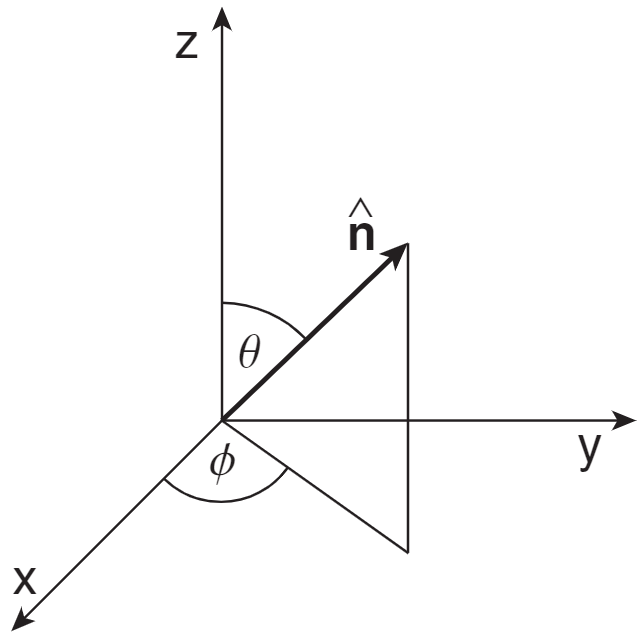
\includegraphics[width=2in]{234.PNG}\end{center} \[\hat{\mathrm n}=\sin(\theta)\cos(\phi)\hat{\mathrm x}+\sin(\theta)\sin(\phi)\hat{\mathrm y}+\cos(\theta)\hat{\mathrm z}\] and \[\vec{S}=S_x\hat{\mathrm x}+S_y\hat{\mathrm y}+S_z\hat{\mathrm z}\] where \(S_x\), \(S_y\), and \(S_z\) are the three components of the spin-\(\frac 1 2\) operator.}
            \begin{enumerate}[label=\textbf{(\alph*)}]
                \item{
                    \textbf{\boldmath Show that \[S_n=\frac{\hbar}{2}\begin{bmatrix}\cos\theta & \sin(\theta)e^{-i\phi} \\ \sin(\theta)e^{i\phi} & -\cos\theta\end{bmatrix}.\]}
                    \vspace*{-12pt}
                    \begin{align*}
                        S_n&=\mathbf{S}\cdot\mathbf{\hat n} \\
                        &=S_x\sin(\theta)\cos(\phi)+S_y\sin(\theta)\sin(\phi)+S_z\cos(\theta)
                    \end{align*}
                    \begin{equation*}
                        S_x=\frac \hbar 2 \begin{bmatrix}0 & 1 \\ 1 & 0\end{bmatrix}\qquad
                        S_y=\frac \hbar 2 \begin{bmatrix}0 & -i \\ i & 0\end{bmatrix}\qquad
                        S_z=\frac \hbar 2 \begin{bmatrix}1 & 0 \\ 0 & -1\end{bmatrix}
                    \end{equation*}
                    \begin{align*}
                        S_n&=\frac \hbar 2 \left(\begin{bmatrix}0 & \sin\theta\cos\phi \\ \sin\theta\cos\phi & 0\end{bmatrix}+\begin{bmatrix}0 & -i\sin\theta\sin\phi \\ i\sin\theta\sin\phi & 0\end{bmatrix}+\begin{bmatrix}\cos\theta & 0 \\ 0 & -\cos\theta\end{bmatrix}\right) \\
                        &=\frac \hbar 2 \begin{bmatrix}\cos\theta & \sin\theta\cos\phi-i\sin\theta\sin\phi \\ \sin\theta\cos\phi+i\sin\theta\sin\phi & -\cos\theta\end{bmatrix} \\
                        &=\frac \hbar 2 \begin{bmatrix}\cos\theta & \sin\theta(\cos\phi-i\sin\phi) \\ \sin\theta(\cos\phi+i\sin\phi) & -\cos\theta\end{bmatrix} \\
                        &=\frac \hbar 2 \begin{bmatrix}\cos\theta & \sin(\theta)e^{-i\phi} \\ \sin(\theta)e^{i\phi} & -\cos\theta\end{bmatrix} \\
                    \end{align*}
                }
                \item{
                    \textbf{\boldmath Show that the eigenvalues of \(S_n\) are \(\pm\frac{\hbar}{2}\), as expected from the S-G experiment.}
                    \begin{align*}
                        (S_n-\lambda I)\ket{\psi}&=\mathbf{0} \\
                        \left(\frac \hbar 2 \begin{bmatrix}\cos\theta & \sin(\theta)e^{-i\phi} \\ \sin(\theta)e^{i\phi} & -\cos\theta\end{bmatrix}-\begin{bmatrix}\lambda & 0 \\ 0 & \lambda\end{bmatrix}\right)\ket{\psi}&=\mathbf{0} \\
                        \begin{vmatrix}\frac \hbar 2 \cos\theta-\lambda & \frac \hbar 2 \sin(\theta)e^{-i\phi} \\ \frac \hbar 2 \sin(\theta)e^{i\phi} & -\frac \hbar 2 \cos\theta-\lambda\end{vmatrix}&=0 \\
                        -\left(\tfrac \hbar 2 \cos\theta-\lambda\right)\left(\tfrac \hbar 2 \cos\theta+\lambda\right)-\left(\tfrac \hbar 2 \sin\theta\right)^2\left(e^{i\phi-i\phi}\right)&=0 \\
                        -\left(\tfrac \hbar 2 \cos\theta\right)^2+\lambda^2-\left(\tfrac \hbar 2 \sin\theta\right)^2&=0 \\
                        \lambda^2&=\left(\tfrac \hbar 2 \cos\theta\right)^2+\left(\tfrac \hbar 2 \sin\theta\right)^2 \\
                        &=\left(\frac \hbar 2\right)^2 \\
                        \lambda&=\pm\frac \hbar 2
                    \end{align*}
                }
                \item{
                    \textbf{\boldmath Show that the eigenvectors of \(S_n\) can be represented as \begin{gather*}\ket{+}_n=\cos\left(\tfrac \theta 2\right)\ket{+}+\sin\left(\tfrac \theta 2\right)e^{i\phi}\ket{-} \\ \ket{-}_n=\sin\left(\tfrac \theta 2\right)\ket{+}-\cos\left(\tfrac \theta 2\right)e^{i\phi}\ket{-}\end{gather*}}%
                    The eigenvector \(\ket \psi\) corresponding to the eigenvalue \(\lambda=+\frac \hbar 2\) is \(\ket{+}_n\), and the eigenvector \(\ket \psi\) corresponding to the eigenvalue \(\lambda=-\frac \hbar 2\) is \(\ket{-}_n\).
                    \begin{align*}
                        (S_n-\lambda I)\ket{\psi}&=\mathbf{0} \\
                        \left(\frac \hbar 2 \begin{bmatrix}\cos\theta & \sin(\theta)e^{-i\phi} \\ \sin(\theta)e^{i\phi} & -\cos\theta\end{bmatrix}-\frac \hbar 2 \begin{bmatrix}1 & 0 \\ 0 & 1\end{bmatrix}\right)\ket{+}_n&=\mathbf{0} \\
                        \begin{bmatrix}\cos\theta-1 & \sin(\theta)e^{-i\phi} \\ \sin(\theta)e^{i\phi} & -\cos\theta-1\end{bmatrix}\ket{+}_n&=\mathbf{0}
                    \end{align*}
                    \begin{align*}
                        \begin{amatrix}{2}\cos\theta-1 & \sin(\theta)e^{-i\phi} & 0 \\ \sin(\theta)e^{i\phi} & -\cos\theta-1 & 0\end{amatrix}
                        \xrightarrow{R_2-\frac{\sin(\theta)e^{i\phi}}{\cos\theta-1}R_1}
                        &\begin{amatrix}{2}\cos\theta-1 & \sin(\theta)e^{-i\phi} & 0 \\ 0 & -\cos\theta-1-\frac{(\sin(\theta)e^{-i\phi})(\sin(\theta)e^{i\phi})}{\cos\theta-1} & 0\end{amatrix} \\
                        \sim
                        &\begin{amatrix}{2}\cos\theta-1 & \sin(\theta)e^{-i\phi} & 0 \\ 0 & -\frac{(\cos\theta+1)(\cos\theta-1)}{\cos\theta-1}-\frac{\sin^2(\theta)}{\cos\theta-1} & 0\end{amatrix} \\
                        \sim
                        &\begin{amatrix}{2}\cos\theta-1 & \sin(\theta)e^{-i\phi} & 0 \\ 0 & -\frac{\cos^2(\theta)-1+\sin^2(\theta)}{\cos\theta-1} & 0\end{amatrix} \\
                        \sim
                        &\begin{amatrix}{2}\cos\theta-1 & \sin(\theta)e^{-i\phi} & 0 \\ 0 & 0 & 0\end{amatrix}
                    \end{align*}
                    If \(\ket{+}_n=a\ket{+}+b\ket{-}\), then the above matrix corresponds to the equation
                    \begin{align*}
                        (\cos\theta-1)a+\sin(\theta)e^{-i\phi}b&=0 \\
                        (1-\cos\theta)a&=\sin(\theta)e^{-i\phi}b \\
                        \sin^2\left(\tfrac \theta 2 \right)a&=\frac 1 2 \sin(\theta)e^{-i\phi}b \\
                        \sin^2\left(\tfrac \theta 2 \right)e^{i\phi}a&=\sin(\theta)\cos^2\left(\tfrac \theta 2 \right)b
                    \end{align*}
                    So \(\ket{+}_n=\sin^2\left(\tfrac \theta 2 \right)e^{i\phi}\ket{+}+\sin(\theta)\cos^2\left(\tfrac \theta 2 \right)\ket{-}\).
                    \par
                    \textit{(I couldn't get the equation to match the form above.)}
                }
                \item{
                    \textbf{\boldmath For which values of \(\theta\) and \(\phi\) does the state \(\ket{+}_n\) reduce to \(\ket{+}_x\) and \(\ket{+}_y\)?}
                    \par
                    \(\ket{+}_x\) was \(\frac{1}{\sqrt 2}(\ket{+}+\ket{-})\), so for \(\ket{+}_n\) to equal \(\ket{+}_x\), we must set \[\cos\frac \theta 2=\frac{1}{\sqrt 2}\] and \[\sin\left(\frac \theta 2\right)e^{i\phi}=\frac{1}{\sqrt 2}.\] Starting with the first equation:
                    \begin{align*}
                        \cos\frac \theta 2&=\frac{1}{\sqrt 2} \\
                        \frac \theta 2&=\frac \pi 4 \\
                        \theta&=\frac \pi 2
                    \end{align*}
                    Then the second equation:
                    \begin{align*}
                        \sin\left(\frac \theta 2\right)e^{i\phi}&=\frac{1}{\sqrt 2} \\
                        \frac{1}{\sqrt 2}e^{i\phi}&=\frac{1}{\sqrt 2} \\
                        e^{i\phi}&=1 \\
                        \phi&=0
                    \end{align*}
                    So for \(\ket{+}_n\) to reduce to \(\ket{+}_x\), \(\theta\) must be \(\frac \pi 2\), and \(\phi\) must be 0.
                    \par
                    Next, \(\ket{+}_y\) was \(\frac{1}{\sqrt 2}(\ket{+}+i\ket{-})\), so for \(\ket{+}_n\) to equal \(\ket{+}_y\), we must set \[\cos\frac \theta 2=\frac{1}{\sqrt 2}\] and \[\sin\left(\frac \theta 2\right)e^{i\phi}=i\frac{1}{\sqrt 2}.\] The solution to the first equation we found earlier to be \(\theta=\frac \pi 2\). We then only have to solve the second equation:
                    \begin{align*}
                        \sin\left(\frac \theta 2\right)e^{i\phi}&=i\frac{1}{\sqrt 2} \\
                        \frac{1}{\sqrt 2}e^{i\phi}&=i\frac{1}{\sqrt 2} \\
                        e^{i\phi}&=i \\
                        \phi&=\frac \pi 2
                    \end{align*}
                    So for \(\ket{+}_n\) to reduce to \(\ket{+}_y\), both \(\theta\) and \(\phi\) must be \(\frac \pi 2\).
                }
                \item{
                    \textbf{\boldmath Suppose that a measurement of \(S_z\) is carried out on a particle in the \(\ket{-}_n\) state. What is the probability that the measurement yields:}
                    \begin{enumerate}[label=\textbf{(\roman*)}]
                        \item{
                            \textbf{\boldmath \(\frac \hbar 2\)?}
                            \par
                            The probability is:
                            \begin{align*}
                                \abs{\braket{+|-}_n}^2&=\abs{\bra{+}\left(\sin\left(\tfrac \theta 2\right)\ket{+}-\cos\left(\tfrac \theta 2\right)e^{i\phi}\ket{-}\right)}^2 \\
                                &=\abs{\sin\left(\tfrac \theta 2\right)}^2 \\
                                &=\sin^2\left(\tfrac \theta 2\right)
                            \end{align*}
                        }
                        \item{
                            \textbf{\boldmath \(-\frac \hbar 2\)?}
                            \par
                            The probability is:
                            \begin{align*}
                                \abs{\braket{-|-}_n}^2&=\abs{\bra{-}\left(\sin\left(\tfrac \theta 2\right)\ket{+}-\cos\left(\tfrac \theta 2\right)e^{i\phi}\ket{-}\right)}^2 \\
                                &=\abs{-\cos\left(\tfrac \theta 2\right)e^{i\phi}}^2 \\
                                &=\cos^2\left(\tfrac \theta 2\right)
                            \end{align*}
                        }
                    \end{enumerate}
                }
            \end{enumerate}
        }
        \pagebreak
        \item{
            \textbf{\boldmath \uline{Three Stern-Gerlach Analyzers with Arbitrary Direction} \\ A beam of spin-\(\frac 1 2\) particles is sent through a series of three S-G analyzers, as shown in the figure. The second S-G analyzer is aligned along the \(\hat{n}\)-direction. \begin{center}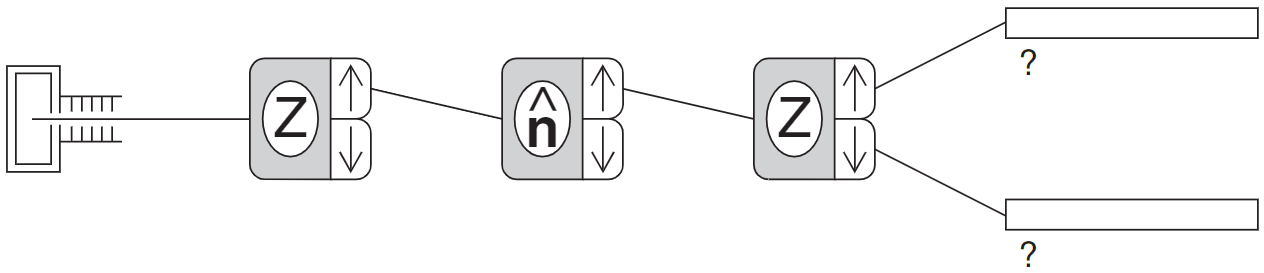
\includegraphics[width=5in]{235.PNG}\end{center}}
            \begin{enumerate}[label=\textbf{(\alph*)}]
                \item{
                    \textbf{Find the probability that particles transmitted through the first S-G analyzer are measured to have spin down at the third S-G analyzer.}
                    \par
                    This would be the probability of the particles going through the first two analyzers multiplied by the probability of those particles going through the third analyzer.
                    \begin{align*}
                        \abs{\braket{+|+}_n}^2\abs{\prescript{}{n}{\braket{+|-}}}^2&=\abs{\bra{+}\left(\cos\left(\tfrac \theta 2\right)\ket{+}+\sin\left(\tfrac \theta 2\right)e^{i\phi}\ket{-}\right)}^2\abs{\left(\cos\left(\tfrac \theta 2\right)\bra{+}+\sin\left(\tfrac \theta 2\right)e^{-i\phi}\bra{-}\right)\ket{-}}^2 \\
                        &=\abs{\cos\left(\tfrac \theta 2\right)}^2\abs{\sin\left(\tfrac \theta 2\right)e^{-i\phi}}^2 \\
                        &=\cos^2\left(\tfrac \theta 2\right)\sin^2\left(\tfrac \theta 2\right) \\
                        &=\frac{\sin^2\theta}{4}
                    \end{align*}
                }
                \item{
                    \textbf{\boldmath How must the angle \(\theta\) of the second S-G analyzer be oriented so as to maximize the probability that particles are meaured to have spin down at the third S-G analyzer? What is this maximum fraction?}
                    \par
                    Since the maximum of \(\sin\theta\) is 1, we mush find a \(\theta\) which will set the probability to \(\frac 1 4\):
                    \begin{align*}
                        \frac{\sin^2\theta}{4}&=\frac 1 4 \\
                        \sin^2\theta&=1 \\
                        \theta&=\frac \pi 2
                    \end{align*}
                    In other words, the second analyzer must be oriented along the \(xy\)-plane, and the maximum probability is \(\frac 1 4\).
                }
            \end{enumerate}
        }
        \pagebreak
        \item{
            \textbf{\boldmath \uline{State Tomography} \\ It is known that there is a 90\% probability of obtaining \(S_z=\frac \hbar 2\) if a measurement of \(S_z\) is carried out on a spin-\(\frac 1 2\) particle. In addition, it is known that there is a 20\% probability of obtaining \(S_y=\frac \hbar 2\) if a measurement of \(S_y\) is carried out. Determine the spin state of a particle as completely as possible from this information. What is the probability of obtaining \(S_x=-\frac \hbar 2\) if a measurement of \(S_x\) is carried out?}
            \par
            From the first criterion:
            \begin{align*}
                \abs{\braket{+|\psi}}^2&=\tfrac{9}{10} \\
                \abs{\braket{+|\psi}}&=\tfrac{3}{\sqrt{10}}
            \end{align*}
            If \(\ket\psi=a\ket{+}+b\ket{-}\):
            \begin{align*}
                \abs{\bra{+}(a\ket{+}+b\ket{-})}&=\tfrac{3}{\sqrt{10}} \\
                \abs{a}&=\tfrac{3}{\sqrt{10}} \\
                a&=\frac{3}{\sqrt{10}}e^{i\alpha}
            \end{align*}
            And from the second criterion: 
            \begin{align*}
                \abs{\prescript{}{y}{\braket{+|\psi}}}^2&=\frac 1 5 \\
                \abs{\prescript{}{y}{\braket{+|\psi}}}^2&=\frac 1 5 \\
                \abs{\tfrac{1}{\sqrt 2}(\bra{+}-i\bra{-})(a\ket{+}+b\ket{-})}^2&=\frac 1 5 \\
                \abs{\tfrac{1}{\sqrt 2}(a-bi)}^2&=\frac 1 5 \\
                \frac 1 2 (\abs{a}^2+\abs{b}^2+ab^*i-a^*bi)&=\frac 1 5 \\
                1+ab^*i-a^*bi&=\frac 2 5 \\
                a\abs{b}e^{-i\beta}i-a^*\abs{b}e^{i\beta}i&=-\frac 3 5 \\
                \abs{b}\left(ae^{-i\beta}-a^*e^{i\beta}\right)&=\frac{3i}{5} \\
                \abs{a}\abs{b}\left(e^{i\alpha}e^{-i\beta}-e^{-i\alpha}e^{i\beta}\right)&=\frac{3i}{5} \\
                \abs{a}\abs{b}\left(e^{i(\alpha-\beta)}-e^{i(\beta-\alpha)}\right)&=\frac{3i}{5}
            \end{align*}
            Arbitrarily set \(\beta=0\):
            \begin{align*}
                \abs{a}\abs{b}\left(e^{i\alpha}-e^{-i\alpha}\right)&=\frac{3i}{5} \\
                \abs{b}\left(e^{i\alpha}-e^{-i\alpha}\right)&=\frac{3\sqrt{10}i}{15} \\
                b&=\frac{\sqrt{10}i}{5\left(e^{i\alpha}-e^{-i\alpha}\right)}
            \end{align*}
            So \(\ket\psi=\frac{3}{\sqrt{10}}e^{i\alpha}\ket{+}+\frac{\sqrt{10}i}{5\left(e^{i\alpha}-e^{-i\alpha}\right)}\ket{-}\).
            \par
            Now, we find the probability of measuring \(S_x=-\frac \hbar 2\):
            \begin{align*}
                \abs{\prescript{}{x}{\braket{-|\psi}}}^2&=\abs{\frac{1}{\sqrt 2}(\bra{+}-\bra{-})\left(\frac{3}{\sqrt{10}}e^{i\alpha}\ket{+}+\frac{\sqrt{10}i}{5\left(e^{i\alpha}-e^{-i\alpha}\right)}\ket{-}\right)}^2 \\
                &=\abs{\frac{1}{\sqrt 2}\left(\frac{3}{\sqrt{10}}e^{i\alpha}-\frac{\sqrt{10}i}{5\left(e^{i\alpha}-e^{-i\alpha}\right)}\right)}^2 \\
            \end{align*}
        }
    \end{enumerate}
\end{document}
